\chapter{Rates of reactions}
\section{How fast?}
\subsection{Order, rate equation and rate reactions}
\paragraph{Rate of reaction is measured} by observing \textbf{changes in quantity over time} e.g. cm$^3 s^{-1} $. In this chapter, you will mainly be dealing with concentration, so knowing the standard unit for it is important(mol $ dm^{-3}$).
\paragraph{Chemists use shorthand} to describe the concentration of compounds. This notation is [A], where A is the compound, and the square brackets mean 'concentration of'.
\begin{equation}
Rate \propto [A]^n - \textnormal{rate is directly proportional to the concentration of A}
\end{equation}
\subsection{Orders of reaction}
\paragraph{The rate of reaction}will often increase as the concentration is increased. It is directly proportional to the concentration raised to a power i.e.
\begin{equation}
rate\propto [A]^n
\end{equation}
The power is the order of reaction with respect to the concentration of the compound.
\subsubsection{Zero order}
\paragraph{This is when}\ch{rate=[A]^0}, meaning that a change in concentration has no effect on the rate of reaction. This is due to anything to the power of 0=1. 
\subsubsection{First order}
\paragraph{This is when}\ch{rate=[A]^1}. Essentially, what happens to the concentration happens to the rate i.e. concentration x2 means rate x2.
\subsubsection{Second order}
\paragraph{This is when}\ch{rate=[A]^2}.So when concentration doubles, rate x$2^2=4$. Basically the rate is the square of the change in concentration.
\subsection{Rate equation and rate constant}
\paragraph{The rate equation is}$rate=k[A]^n[B]^m$. The overall order can be found by adding the powers together. When a question says both concentrations are changed, you use the overall order to find the rate.
\paragraph{The units of the rate constant}are usually \ch{moldm^{-3}s^{-1}}. However,this can be derived by rearranging the rate equation to make k the subject as this is the rate constant. It is useful to remember that the concentrations are measured in \ch{moldm^{-3}}.
\subsection{Determining orders from experimental results}
\paragraph{The best way}to learn this is by doing past paper question. Some great resources can be found on: pastpapers.com; physicsandmathstutor.co.uk or http://www.a-levelchemistry.co.uk/.
\paragraph{The questions}will usually contain a table with the headings: Experiment, Concentration of respective elements and the initial rate. The way to go about these questions is by first seeing how the concentration change between experiments e.g. x2. Then look at initial rate. See how this changes to determine the rate e.g. if it's x4, this would be second order.
\begin{center}
\includegraphics[scale=0.5]{workedorder.png}
\end{center}
\newpage
\section{Concentration-time graph}
\paragraph{You can measure rates}by looking for a \textbf{change} in mass or by gas collection in a certain \textbf{time}. You can also use a colorimeter if some of the compounds are coloured.
\subsection{Concentration-time graph}
\paragraph{The gradient of the concentration-time graph} is the rate of reaction.The order of reaction can be deduced from the shape of the graph.
\subsubsection{Zero order}
\paragraph{This graph slopes down}i.e. it has a negative gradient. The line is straight meaning that the rate is constant as concentration falls over time(as reactants used up). The gradient of the line is the rate constant-k.
\subsubsection{First order}
\paragraph{This graph is a downward-sloping curve}.The gradient decreases over time,slowing the reaction down. The \textbf{half-life}( \textit{time taken for concentration to halve}) is constant.
\subsubsection{Second order}
\paragraph{This graph is steeper at the beginning than the first order.}However, it tails off more slowly.
\begin{center}
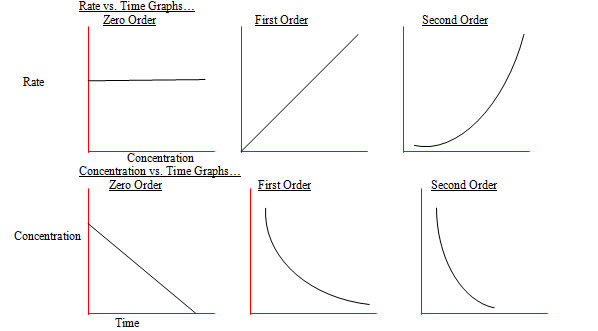
\includegraphics[scale=0.5]{conctimegraphs.png}
\end{center}
\subsection{Half-life}
\paragraph{Half-life,}which can be represented by $t_{1/2}$ is the time taken for half of the reactant to be used up. First order reactions halve the concentration every half life. The curve is exponential, showing \textbf{exponential decay}
\subsubsection{Determination of rate constant from rate}
\paragraph{You can draw a tangent to the curve}on a concentration-time graph.This will give you the rate of reaction. Then, you insert this into your re-arranged rate equation,where k is the subject.This should give you the rate constant, all you need to do is figure out the units.
\paragraph{You can also use an awesome formula:}\begin{equation}
k=\frac{\textnormal{ln}2}{t_{1/2}}
\end{equation}
This method is more accurate than drawing a tangent.
\section{Rate-concentration graphs and initial rates}
\paragraph{Always be careful to check the axes of your graph.}Here, the rate is on the left and concentration along the bottom. Normally, as concentration increases, so does rate due to kinetics i.e. more particles etc. Therefore the curves usually\textbf{slope up} rather than down.
\subsection{Orders from shapes}
\subsubsection{Zero order}
\paragraph{The gradient is 0,}meaning there is no slope. Rate is not affected by a change in concentration( a visual representation of its definition).The y-intercept gives you the rate constant-k.
\subsubsection{First order}
\paragraph{This is a upward-sloping straight-line graph}beginning at the origin. This is because when concentration is 0, rate is zero. The rate constant her is the gradient of the line.
\subsubsection{Second order}
\paragraph{This is an upward sloping curve.}Therefore the gradient constantly increases. It also means that the rate constant cannot be worked out directly by the curve. Instead, you need to \textbf{plot a second graph} of the rate against $[A]^2$ (concentration squared). This will give you a straight line graph through the origin, where the gradient is k.
\subsection{Initial rates method}
\paragraph{The initial rate}is the instantaneous rate when t=0.It can be measured by drawing a tangent where t=0 on a concentration-time graph.It can be obtained by separate experiments using different concentrations of one of the reactants.Clock reactions are an approximation of this method.
\paragraph{A clock reaction}is a convenient method of obtaining the initial rate. It is done by measuring time from the beginning of an experiment to a visual change. This change will often be a precipitate or colour.
\paragraph{As long} as there isn't a significant change in rate, it's assumed that the average rate of reaction is equal to the initial rate. The initial rate is then proportional to \frac{1}{t}\. 
      The experiment is then repeated with different concentrations and values of \frac{1}{t}\ are calculated each time.
\paragraph{Iodine clock reactions} are simple and you've probably done this as a PAG. You mix together sodium thiosulphate, starch and iodine. The endpoint of the reaction is when a blue-black colour appears- as iodine racts with starch as soon as the Sodium thiosulphate is used up.
\subsection{The rate determining step}
\paragraph{Given the stoichiometry} of chemical reactions, some are very unlikely to be completed in one step. In fact, there is probably more than one, the \textit{slowest} being called the \textbf{rate determining step}\footnote{I shall now refer to this as RDS}.
\paragraph{An example}would be the reaction:
\ch{H2O2 + HI -> H2O +I2}
As the ionic equation is \ch{H2O2 + 2I- +2H+ -> I2 + 2H2O}, all the ions would have to collide at the same time for the reaction to take place in one step. 
	The following is the most likely to happen:
\ch{H2O2 + HI -> H2O + HOI} SLOW(RDS) and then
\ch{HOI + HI -> H2O + I2} FAST.
\paragraph{A good way}to ensure you get full marks in finding ) possible steps in a reaction mechanism
from the rate equation is to use the powers in the rate equation to work out the stoichiometry.
\paragraph{For example}if the rate equation is:
 \begin{equation}
 rate=k[NO_2]^2
 \end{equation}
 And you are given the overall balanced equation- \ch{NO2 + CO -> NO +CO2}, you know that two molecules of \ch{NO2} are involved in the RDS. Therefore,
 \ch{2NO2 -> NO + NO3} SLOW(RDS) and then
\ch{NO3 + CO -> NO2 + CO2 } FAST
\subsection{The effect of temperature on rate constants}
\paragraph{At a constant temperature}, K is constant and does not change due to changes in pressure, temperature or the presence of a catalyst. This is because the position of equilibrium will shift to nullify the change. Only temperature has an effect on the equilibrium constant.
\subsubsection{Exothermic reactions}
\paragraph{If the forward reaction}is exothermic, K(the equilibrium constant) \textbf{decreases} with increased temperature. Raising the temperature also decreases yield of products and increases that of reactants. Applying this to questions is relatively easy and I will not go further into detail.
\subsubsection{Endothermic reactions}
\paragraph{If the forward reaction}is endothermic, K(the equilibrium constant) \textbf{increases} with increased temperature. Raising the temperature also increases yield of products and decreases that of reactants.
[ARRHENIUS EQUATION PIC FOM BOOK P 289 & 290]
\section{How far?}
\paragraph{Partial pressure}is the contribution of a gas towards the total gas pressure.
\(Partial pressure=mole fraction* total pressure\). Partial pressure is always measured in kPa. It is also good to know that the sum of partial pressures is equal to the total pressure.
\paragraph{An example}:
A gas mixture with total pressure 320000Pa contains 2 mol of \ch{N2} and 3 mol of \ch{O2}. Find their partial pressure.
\begin{itemize}
\item Find the mole fractions
\ch{N2} makes up 2 mol/5mol of gas and \ch{O2} makes up 3/5 moles.
\item Convert Pa to kPa: 320000Pa= 320kPa
\item Multiply the fraction by the total pressure
0.4*320= 128 kPa and 0.6*320= 192kPa 
\end{itemize}
\paragraph{The equation}for K$_p$ is the same as K$_c$, however, instead of square brackets, you do this p(X), where X is a chemical in gaseous form. It is important to note that you omit any non-gases from the equation or expression. Also, units are worked out in the same way as in K$_c$, but please note that the k in kPa is not involved in deducing units.